\section{全线圈验证与空间杆控制转移}
\label{sec:physical-results}

\subsection{能量一致的磁力仍可能否定仿射植物模型}
先对线圈接口进行独立核查，再评价控制。最终线圈核与力分配器中，几何虚功与磁能求导所得力的正则范数差为 $4.44\times10^{-16}$。沿十二个方向、以 $2\times10^{-6}$ 和 $10^{-6}$ 扰动进行能量差分，误差分别为 $3.70\times10^{-10}$ 和 $7.04\times10^{-10}$。圆环轴上场闭式解将绝对 SI 单位核验到 $3.90\times10^{-16}$ 的相对误差；采样散度与旋度缺陷小于 $1.58\times10^{-17}$\,T\,m$^{-1}$。圆线圈求积由 128 加密至 256、512 点，力变化至多 $3.69\times10^{-16}$。这些局部浮点检查支持实现中的能量/力一致性，但不构成连续工作域认证。

尽管如此，全线圈力仍与具有相同原点场、梯度和总电流的仿射场存在显著差异。表~\ref{tab:coil-quadrature} 和图~\ref{fig:coil} 在同一物理 Ritz 系数下比较，并将各网格力统一拉回 20 单元正则坐标。约 98.6\% 的相对差异随空间加密仍然存在，因此不能用导线积分误差或粗网格只有一个磁积分点来解释。相邻空间网格的全力绝对差仍为 $0.00586672$ 和 $0.00145763$，20 单元近似尚未空间收敛。数值秩的增加也表明，应实际测量依赖求积的可达性，而不能从电流通道数推断。

\begin{table}[t]
\centering
\caption{共同位形下的线圈力与可达性诊断。相对力误差为 $\|F_{\rm full}-F_{\rm affine}\|/\|F_{\rm full}\|$；电流端口秩采用相对阈值 $10^{-8}$。}
\label{tab:coil-quadrature}
\begin{tabular}{@{}rrrr@{}}
\toprule
\shortstack{空间\\单元} & \shortstack{磁积分\\点} & \shortstack{相对\\力误差} & \shortstack{$G_I$\\的秩}\\
\midrule
20 & 1 & 0.985235663 & 5\\
40 & 2 & 0.985978752 & 7\\
80 & 4 & 0.986182968 & 7\\
\bottomrule
\end{tabular}
\end{table}

\begin{figure*}[t]
\centering
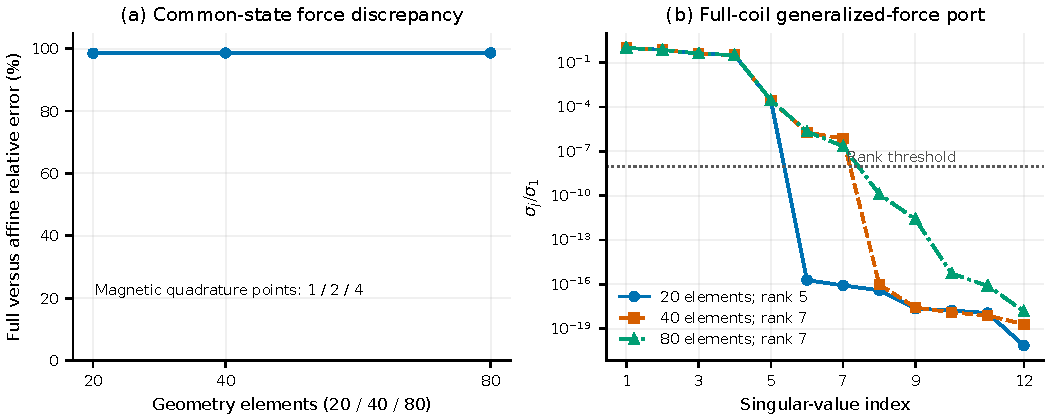
\includegraphics[width=\textwidth]{../figures/coil.pdf}
\caption{20/40/80 个空间求积单元在同一物理 Ritz 系数 $q$ 下的全线圈力差异与电流端口归一化奇异值。所有力和端口均使用共同的 20 单元正则基，磁求积分别有 1/2/4 个有效点。持续存在的约 98.6\% 仿射差异，以及相对阈值 $10^{-8}$ 下 5/7/7 的数值秩，表明不能将十二个线圈通道解释为十二个独立广义力。}
\label{fig:coil}
\end{figure*}

对 $d=0.2P_0$ 和 $0.1$\,ms 分配周期，正交不可达残差为 $2.65530\times10^{-4}$，受限残差为 $4.01583\times10^{-4}$，且 20\,A\,s$^{-1}$ 斜率约束激活。将目标放大 10 倍和 100 倍，受限残差分别为 $0.00500641$ 和 $0.07305644$。正确反馈导数的方向有限差分误差为 $2.40\times10^{-9}$；改为对复合 Hamiltonian 求导会造成 $5.47301$ 的场差，而冻结反馈会漏掉谱范数为 $12.56491$ 的 Jacobian 项。这是两个不同的实现错误，均直接影响隐式闭环更新。

\subsection{实际受限轨迹及其分辨率限制}
受控轨迹由相同 $z_0=\operatorname{initial\_state}(0.01)$、总偏置、材料、增益和约束独立积分得到。取 $\gamma=0.2$，八次控制更新覆盖 $\tau\in[0,0.004]$，即 $0.89733794$\,ms。每周期使用一个或两个 RK4 子步，形成 8 步和 16 步网格。各分支分别计算自身反馈与实际植物力，没有将仿射轨迹复用为全场轨迹。

全植物/全控制器与仿射植物/仿射控制器的最大正则状态范数差为 $3.90705\times10^{-4}$，各自粗细网格差约 $7.22\times10^{-8}$，因此植物近似对轨迹的影响得到分辨。但在同一全植物上，将全场控制器换成仿射控制器仅造成 $7.17555\times10^{-8}$ 的轨迹差。该窗口未分辨出全场控制设计的性能优势。含力补偿在内的四个分支，在细网格上的总能量和机械能--功残差幅值均约为 $6.25\times10^{-11}$。磁点采样场与梯度最大值分别为 $0.501325$\,mT 和 $0.00431404$\,T\,m$^{-1}$。力补偿达到 20\,A\,s$^{-1}$，但仍留下约 $4.01416\times10^{-4}$ 的最大力残差。

最终分配器从经独立验证可行的上一电流启动力目标优化。真实重跑相较此前成功的补偿轨迹，状态最大差为 $1.17\times10^{-12}$，电流最大差为 $6.51\times10^{-10}$\,A。该一致性并不证明优化算法具有相同导数。严格匹配初始偏置后重新计算的 36 维采样映射，共点投影与力补偿的数值秩分别为 28 和 36，在所用正则/电流坐标中的条件数分别为 $5.43\times10^{18}$ 和 $2.09\times10^5$。机械子块相对于 $K_0$ 的缺陷分别为 $3.22749\times10^{-3}$ 和 $1.03008\times10^{-4}$。尽管机械终态差仅 $1.04\times10^{-14}$，新旧力分配 Jacobian 的谱范数差仍为 $1.77112\times10^{-4}$，主要来自电流输出块。因此，可行分配成功和轨迹几乎相同，并不证明采样映射光滑、可逆或辛。

\subsection{环境模型转移：执行可行但跟踪未改善}
\begin{figure*}[t]
\centering
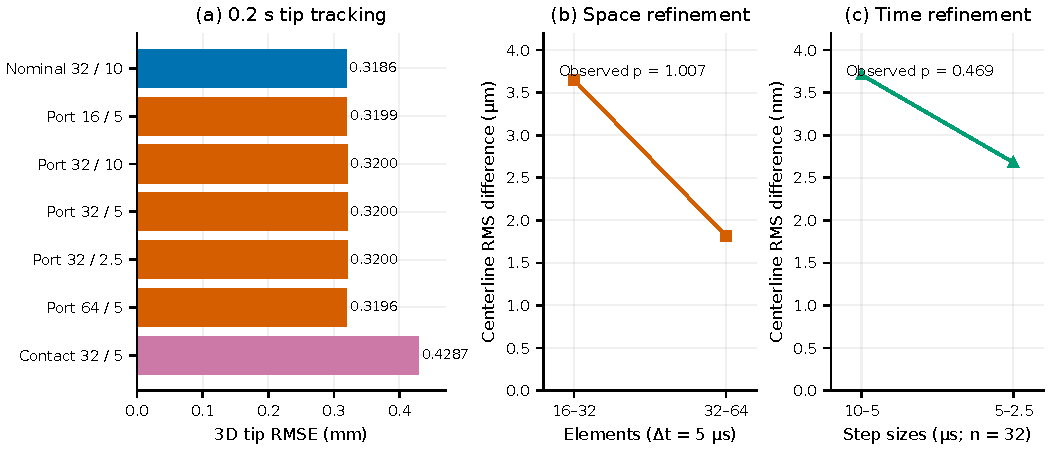
\includegraphics[width=\textwidth]{../figures/rod.pdf}
\caption{空间杆在 0.2\,s 内的控制转移。(a) 标签依次给出单元数和以微秒计的步长；名义控制与端口控制的公平比较采用 32 单元、10\,$\mu$s。接触算例使用独立的 1.6\,mm 半径管腔几何，其余算例采用标称 3\,mm 管腔。(b,c) 为共同输出时刻、129 个参考弧长点上的相邻中心线差异。观察阶描述这些数值差异，并不建立精确 PDE 误差或时间二阶收敛。}
\label{fig:rod}
\end{figure*}
七个空间杆算例采用全线圈力和式 \eqref{eq:port-units} 的物理增益，从直杆静止状态及零实际电流开始积分 $0.2$\,s。此时 $0.3$\,s 的目标斜坡仍未完成。程序使用 PyElastica PositionVerlet，并加入上述环境载荷。相同的 32 单元、10\,$\mu$s 网格上，名义控制末端 RMSE 为 $0.318558$\,mm，加入端口反馈后为 $0.320032$\,mm，跟踪略有恶化。32 单元、5\,$\mu$s 端口算例的 RMSE 为 $0.320033$\,mm，最大电流为 $1.67831$\,A，最大斜率为 20\,A\,s$^{-1}$，电流斜坡连接缺陷为零，387 个固定约束采样点上的已记录违例为零。保存节点的全场和梯度最大值分别为 $0.279966$\,mT 和 $0.0223521$\,T\,m$^{-1}$。这些有限样本不构成连续工作域认证。

标称 3\,mm 管腔未激活接触。独立的 1.6\,mm 半径窄管算例初始无穿透，在运动中产生 $61.6032$\,$\mu$m 的最大穿透和 $11.3524$\,$\mu$N 的总法向力，RMSE 为 $0.428689$\,mm。图~\ref{fig:rod} 单独报告这一应力工况。理想端口增量功率非正，但投影后与斜坡起点的增量功率分别达到正值 $3.19262\times10^{-8}$ 和 $3.20376\times10^{-8}$\,W。32 单元、5\,$\mu$s 算例的机械能--功残差为 $1.24636\times10^{-14}$\,J。因此，准确功率计账与实际执行输入失去理想耗散保证可以同时出现。

原分配器的回退曾引入约 $0.133$\,A 的电流差并破坏时间加密结果。最终程序先截到电流盒，再沿上一可行电流出发的线段解析修复，同时保留所有优化器未收敛状态。七个最终算例均无回退、各有 99 次修复及一至四次未收敛状态，故未将可行性等同于已证最优性。在 129 个共同参考弧长点，相邻中心线 RMS 差对 16/32/64 单元为 $3.64802/1.81514$\,$\mu$m，对 10/5/2.5\,$\mu$s 步长为 $3.70928/2.67939$\,nm。观察空间阶与时间阶分别为 $1.00703$ 和 $0.469234$；这些结果既不提供精确 PDE 误差，也未证实时间二阶收敛。

最后，另设 2\,ms 保守比较，匹配初态、材料和固定电流，并同时关闭流体、管壁、重力与阻尼。ROM 与 16/32/64 单元杆的中心线 RMS 差依次增大为 $7.85933$、$11.2030$、$14.1690$\,nm，末端 RMS 差分别为 $33.4755$、$65.6852$、$86.4209$\,nm。Ritz 截断、剪切/伸长约束、求积及基部标架离散仍构成不同模型误差。该固定电流还在全杆上产生 $0.798394$\,T\,m$^{-1}$ 的梯度，超过 $0.03$\,T\,m$^{-1}$ 限值。因此该诊断不是可行导航结果，也不是已收敛的 ROM 误差证书。
